\let\negmedspace\undefined
\let\negthickspace\undefined
\documentclass[journal]{IEEEtran}
\usepackage[a5paper, margin=10mm, onecolumn]{geometry}
%\usepackage{lmodern} 
\usepackage{tfrupee} 

\setlength{\headheight}{1cm} 
\setlength{\headsep}{0mm}     

\usepackage{gvv-book}
\usepackage{gvv}
\usepackage{cite}
\usepackage{amsmath,amssymb,amsfonts,amsthm}
\usepackage{algorithmic}
\usepackage{graphicx}
\usepackage{textcomp}
\usepackage{xcolor}
\usepackage{txfonts}
\usepackage{listings}
\usepackage{enumitem}
\usepackage{mathtools}
\usepackage{gensymb}
\usepackage{comment}
\usepackage[breaklinks=true]{hyperref}
\usepackage{tkz-euclide} 
\usepackage{listings}                                        
\def\inputGnumericTable{}                                 
\usepackage[latin1]{inputenc}                                
\usepackage{color}                                            
\usepackage{array}                                            
\usepackage{longtable}                                       
\usepackage{calc}                                             
\usepackage{multirow}                                         
\usepackage{hhline}                                           
\usepackage{ifthen}                                           
\usepackage{lscape}

\begin{document}

\bibliographystyle{IEEEtran}
\vspace{3cm}

\title{5.11.2}
\author{AI25BTECH11003 - Bhavesh Gaikwad}
{\let\newpage\relax\maketitle}

\renewcommand{\thefigure}{\theenumi}
\renewcommand{\thetable}{\theenumi}
\setlength{\intextsep}{10pt} 


\numberwithin{equation}{enumi}
\numberwithin{figure}{enumi}
\renewcommand{\thetable}{\theenumi}


\textbf{Question}: Determine the current in each branch of the network shown in Fig.01
\begin{figure}[htbp]
    \centering
    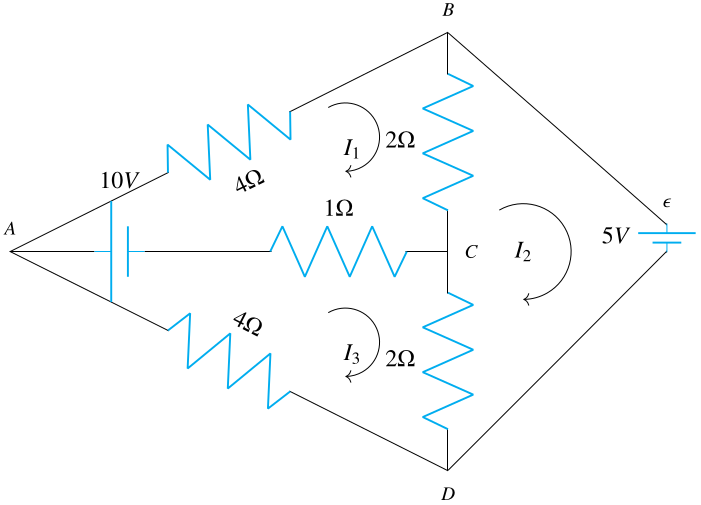
\includegraphics[width=\columnwidth]{figs/figQ.png}
    \caption{}
    \label{fig:figs/fig1.png}
\end{figure}

\newpage

\textbf{Solution:}\\

Using mesh current analysis with Kirchhoff's Voltage Law (KVL) to solve the question.\\


Applying KVL to the loop ABCA,
\begin{equation}
-7I_1 + 2I_2 + I_3 = -10
\end{equation}


Applying KVL to the loop CBDC,
\begin{equation}
2I_1 - 4I_4 + 2I_3 = -5
\end{equation}

Applying KVL to the loop ACDA,
\begin{equation}
-I_1 - 2I_2 + 7I_3 = 10    
\end{equation}

Therefore, the Three equations are: 
$$ -7I_1 + 2I_2 + I_3 = -10$$
$$2I_1 - 4I_4 + 2I_3 = -5$$
$$-I_1 - 2I_2 + 7I_3 = 10$$\\

Let $\vec{M} = \myvec{-7 & 2 & 1 \\ 2 & -4 & 2 \\ -1 & -2 & 7}$ and $\vec{x} = \myvec{I_1 \\ I_2 \\ I_3}$ and $\vec{T} = \myvec{-10 \\ -5 \\ 10}$\\\\

\begin{equation}
    \therefore \, \vec{M}\vec{x}=\vec{T}
\end{equation}

\begin{center}
OR    
\end{center}

\begin{equation}
    \myvec{-7 & 2 & 1 \\ 2 & -4 & 2 \\ -1 & -2 & 7}\vec{x} = \myvec{-10 \\ -5 \\ 10}
\end{equation}

The Augmented Matrix:
\begin{equation}
\left(
\begin{array}{ccc|c}
     -7 & 2 & 1 & -10  \\
     2 & -4 & 2 & -5 \\
     -1 & -2 & 7 & 10 
\end{array}
\right)
\end{equation}

Row Transformation-1: $R_3 \rightarrow R_3 + R_1$
\begin{equation}
\left(
\begin{array}{ccc|c}
     -7 & 2 & 1 & -10  \\
     2 & -4 & 2 & -5 \\
     -8 & 0 & 8 & 0 
\end{array}
\right)
\end{equation}

Row Transformation-2: $R_2 \rightarrow R_2 + \frac{R_3}{4}$
\begin{equation}
\left(
\begin{array}{ccc|c}
     -7 & 2 & 1 & -10  \\
     0 & -4 & 4 & -5 \\
     -8 & 0 & 8 & 0 
\end{array}
\right)
\end{equation}

Row Transformation-3: $R_3 \rightarrow R_3 - \frac{8R_1}{7} - \frac{4R_1}{7}$
\begin{equation}
\left(
\begin{array}{ccc|c}
     -7 & 2 & 1 & -10  \\
     0 & -4 & 4 & -5 \\
     0 & 0 & 32/7 & -60/7 
\end{array}
\right)
\end{equation}

\bigskip

\begin{equation}
    \myvec{-7 &  2 & 1 \\ 0 & -4 & 4 \\ 0 & 0 & 32/7 }\myvec{I_1 \\ I_2 \\ I_3} = \myvec{-10 \\ -5 \\ -60/7 }
\end{equation}

\bigskip

\begin{equation}
\boxed{\therefore I_1 = 55/56 A, \, I_2 = 5/8 A, \, I_3 = 15/8}
\end{equation}


\end{document}  
